\section{Infrastructure}
\subsection{Domain information}

Here we work our way piece by piece {\bf from rough to detailed} information.
Therefore we first have to get a technical overview of the company. Since we
usually already know the name of the company or even the domain name, this
information is generally sufficient to determine how the company is
structured.
\begin{figure}
  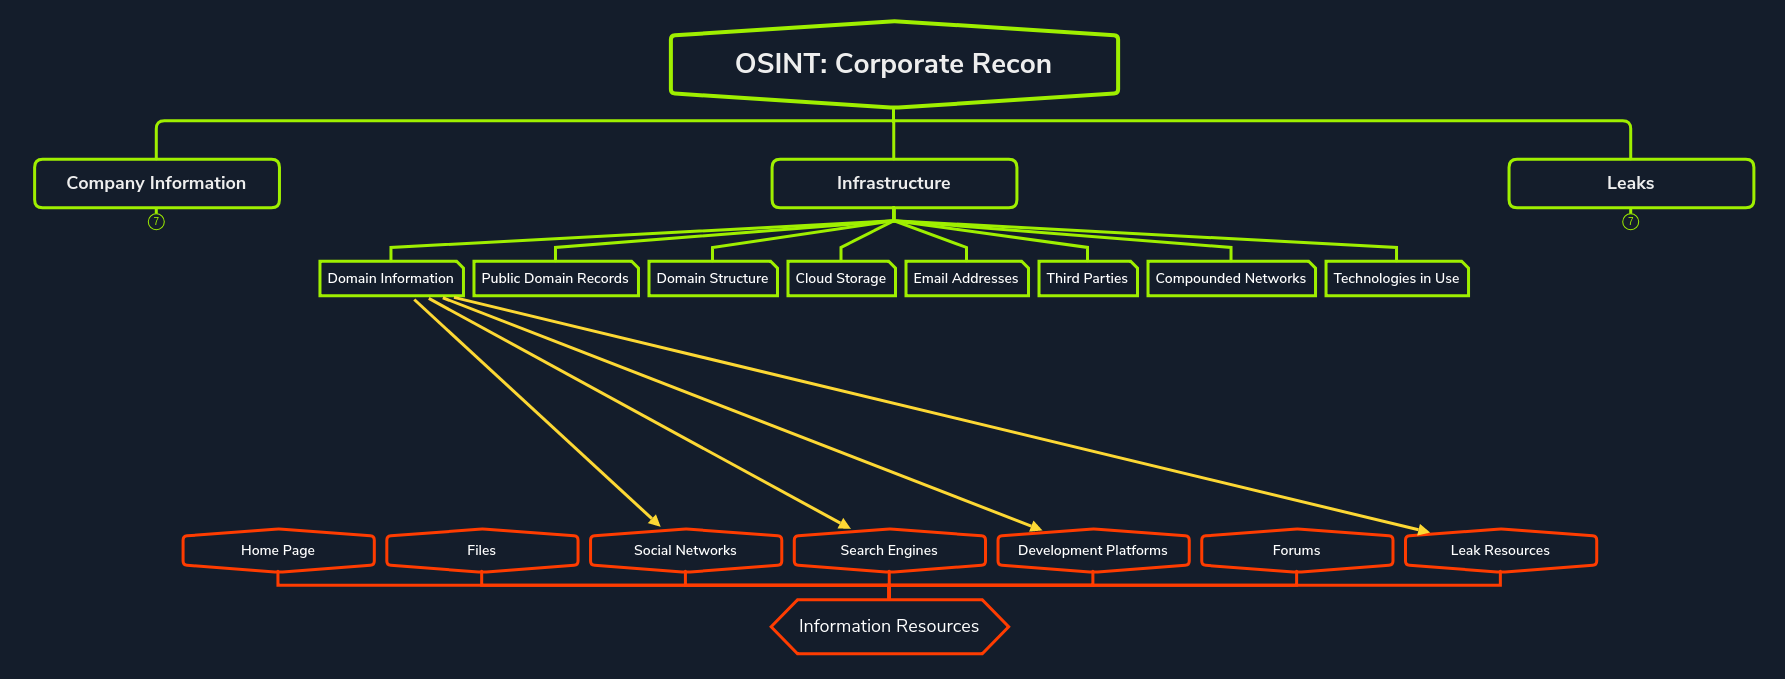
\includegraphics[width=\linewidth]{recon/osint/images/infra-domain-info.png}
  \caption{OSINT Domain information}
  \label{fig:osint-domain-info}
\end{figure}

The element we focus on in the first phase of the company's infrastructure
investigation is the domain names we can find. We then go into each domain and
get an overview of the subordinate structure that contains 
\begin{itemize}
        \item Netblocks
        \item Name Servers
        \item Mail Servers
        \item subdomains
        \item hosts/IP addresses.
\end{itemize}

We can classify the rough structure into three categories:
\begin{itemize}
        \item Public Records:  	
        \item Third Parties 	
        \item Domains
\end{itemize}

\subsubsection{Social Networks}
We often find references to domains or subdomains on social media platforms.


\subsubsection{Search Engines}
One of the most efficient methods of searching for domains is offered by
various search engines. In this case, we cannot focus on a domain name, but we
have to work with general company terms, such as the company name, the name of
the application or service, and others.

Another excellent way to find out information about our target domain is to use
a particular Search Engine Optimization (SEO) field called backlinks. 

One of such backlinks analyzers is
\href{https://app.neilpatel.com/en/seo_analyzer/backlinks}{Ubersuggest}.

\subsubsection{Development Platforms}
Development platforms also offer excellent information resources for us here,
as we will often find code that sometimes even provide information that is
dangerous for the company. This information can range from IP addresses and
hostnames, configuration files to credentials.

\subsubsection{Leak Resources}
Once we have a list of the company's domains, we can use it to look for known
anomalies that affect the company and the corresponding domain. One of the best
sources of information for this is
\href{https://www.virustotal.com/}{VirusTotal}, where we can scan each domain
for suspicious activity.


Another source that searches against many different developer platforms is
\href{https://searchcode.com/}{Searchcode}. It searches all possible codes for
terms that we specify in the search and shows us the sources accordingly.

\subsection{Public Domain Records}

Public domain records offer us excellent opportunities to trace the company's
information technology infrastructure structure. With the right arrangement and
knowledge of what the records are for and what information they contain, they
can provide us with information about the company's Internet presence. To get
this, we need to find out at least four components:
\begin{verbatim}
1. Netblocks / CIDR 	2. ASN 	3. DNS Servers 	4. Mail Servers
\end{verbatim}

This gives us an overview of which systems are accessible from the internet, in
which address range they are located, which IP neighbors they have, and how the
interaction between them takes place.

\begin{figure}
  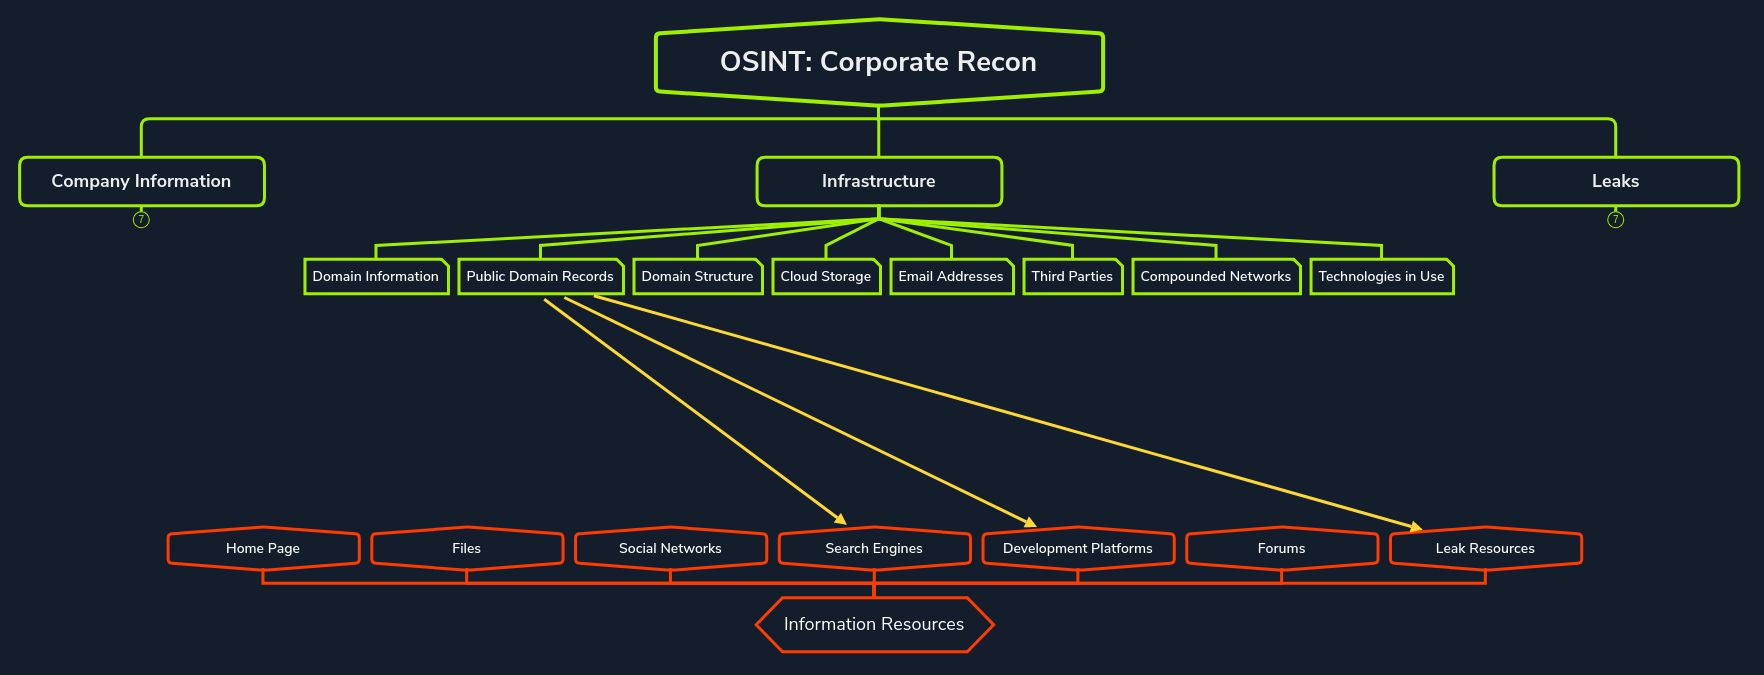
\includegraphics[width=\linewidth]{recon/osint/images/infra-pub-records.png}
  \caption{OSINT Domain public records}
  \label{fig:osint-infra-pub-records}
\end{figure}

\subsubsection{Search Engines}
The minimum information we need to get from our client, apart from the company's
name, is a domain or at least an IP address to start with. The scope of this
can vary greatly.

{\bf 1. Netblocks / CIDR}

During a black-box penetration test, our client will often only provide the
domain name. We can use this to find out a lot of helpful information. First of
all, we should find the IP address of the main webserver(s) and the IP address
range(s) / CIDR. For this, we can use the following command.
\begin{verbatim}
host www.inlanefreight.com
\end{verbatim}
Now that we have the IP address of the web server, we can find out which IP
address range it is located in. By default, we can work with the Whois protocol
used by a distributed database system to retrieve information about internet
domains and IP addresses and their owners.
\begin{verbatim}
whois 134.209.24.248
\end{verbatim}
We can also search the WHOIS databases for the company name. We are often given different identification numbers (mnt-ref), which we can use for further searches. These stand for the maintainer objects, which are used as a reference for the organization objects.
\begin{verbatim}
whois -B --sources RIPE,ARIN target-company
\end{verbatim}
We can also query the individual databases and identify the associated netblocks.
\begin{verbatim}
whois -h whois.arin.net target-company | grep -v "#" | sed -r '/^\s*$/d'
\end{verbatim}
Here is the \href{https://www.arin.net/resources/registry/whois/rws/cli/}{ARIN
list} of other flags we can use to get more information from
the maintainer objects. 


{\bf 2. ASN}

We can also see another crucial piece of information here, the {\bf OrigisAS}.
This is the {\bf Autonomous System Number (ASN)}. This number is unique and is
made publicly available so routing information can be exchanged with other
systems. This is done with specific IP prefixes, which we can use to find out
the netblocks ({\bf public ASNs}). There are also {\bf private ASNs} intended
for systems that only communicate via a provider. Other protocols such as the
{\bf Border Gateway Protocol (BGP)} are used if this is the case. We can use
\href{https://mxtoolbox.com/SuperTool.aspx}{MXToolbox} and its {\bf ASN Lookup}
option with the ASN to find out how many subnets the owner has.

Another way to get more information about the domain is to use the
\href{https://lookup.icann.org/lookup}{ICANN lookup}. Each domain is registered
to an organization or person with a unique ID, which provides information about
when the domain was created and expires.

{\bf 3. DNS Servers}

DNS servers are essential services today because they help the regular user
reach the web services they want.  It is often the case that companies own
several domains, and accordingly, these domains can offer different attack
vectors that can affect each other. The next step is to look at the DNS records
of our target domain using dig. Dig is a DNS lookup utility that can be used to
obtain publicly available information from DNS.

\begin{verbatim}
dig any inlanefreight.com
\end{verbatim}

If we now take a closer look at the records, we see that the SOA record shows
another domain, infreight.com. Therefore we will also look at these if the
scope allows us to do so. In this case, we assume that we have permission to
test this domain as well.

Another source we can use, which gives us a much better representation of the
DNS servers' records, is \url{https://dnsdumpster.com/}{DNSdumpster}.

Here we can see the entries for the respective DNS servers and the locations of
the corresponding hosts and servers. Then we see the respective IP addresses
and corresponding subdomains that could be obtained from the entries.
Additionally, DNSdumpster can sometimes show us the services running on the
server if it can passively identify them. Finally, at the bottom of the page,
we can see a domain map that shows the relationships between the servers
connected with the records.

{\bf 4. Mail Servers}

Mail Server / Exchange server ({\bf MX}) is one of the most critical services
today, as it ensures that our emails reach the desired communication partners.
Other servers use it as an interstation (relay) for sending spam or viruses. It
often happens that MX servers do not only use specially registered servers as
relays. This gives us the possibility to perform an {\bf Open Relay Attack}.

MX servers represent a massive attack vector. There is nothing worse for a
company apart from a complete compromise than the fact that all unencrypted
emails can be intercepted and read. This means that not only GDPR guidelines
have been violated by requiring the company to ensure that customer data is
kept confidential, but it also significantly impacts customer satisfaction and
customer trust, which will be significantly damaged.

\href{https://mxtoolbox.com/}{MXtoolbox} offers an excellent service to test
the MX servers for Open Relay.


\subsubsection{Development Platforms}

Searching for code on developer platforms can bring surprising results. Apart
from already highly sensitive data such as user names and passwords, we can
also find {\bf configuration files} containing the latest administration settings. We
can use \href{https://searchcode.com/}{searchcode} again with specific strings
and known {\bf IP addresses} or {\bf domain names} to get such results.
However, in this case, we need a basic understanding of the configuration
files, how they can look, and which variables can be used for DNS
configuration.

\subsubsection{Domain structure}
Now that we have gathered a lot of information, we need to focus on the
intelligence of this process and create an {\bf overview of the domain}, and
analyze our results. We should take our time because the better we understand
the structure of the domain, the easier it will be to take the appropriate
steps later. Furthermore, we narrow down the goals and seek out the {\bf low
hanging fruit} of all the systems that promise the best possible results for us.


\begin{figure}
  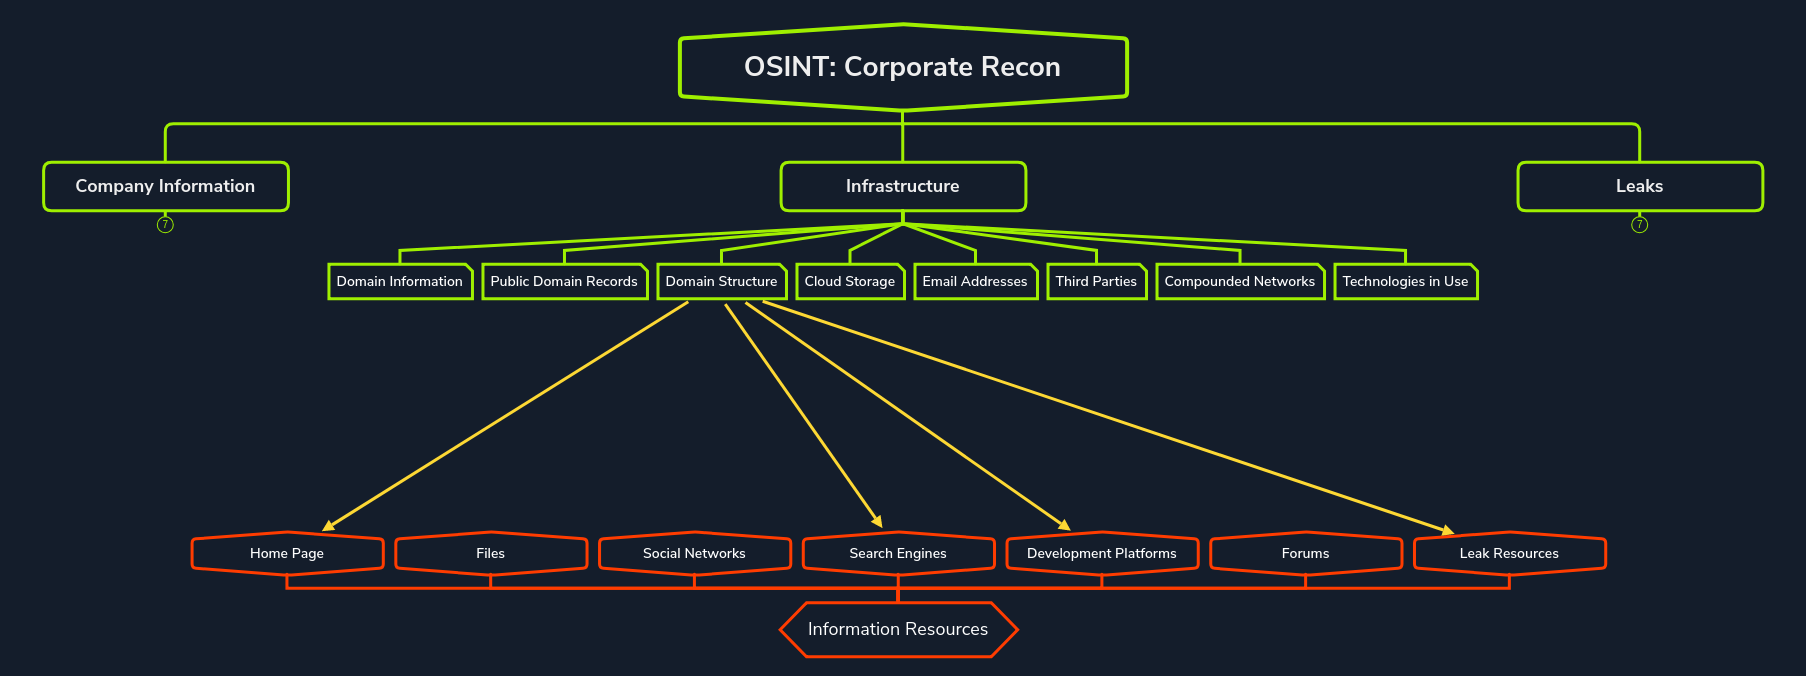
\includegraphics[width=\linewidth]{recon/osint/images/infra-domain-structure.png}
  \caption{OSINT Domain structures}
  \label{fig:osint-infra-domain-structure}
\end{figure}
This preparation can take several hours of study but save us time in the
following steps because we will not test each system blindly, but proceed
methodically, organized and structured. This represents the professionalism of
our work and gives a much better impression in the reports for our customers.

\subsubsection{Home Page}
Countless websites link to other subdomains. Therefore, we should always pay
attention to each clickable area on every web page owned by the company.

\subsubsection{Search Engines}

Since we are still in the passive information gathering phase, we should use
passive techniques to find out more subdomains. For this, we can use a tool
called \href{https://github.com/UnaPibaGeek/ctfr}{CTFR}. It uses Certificate
Transparency logs from
\href{https://www.certificate-transparency.org/}{Certificate Transparency} and
\href{https://crt.sh/}{crt.sh}.

\begin{verbatim}
./ctfr.py -d inlanefreight.com | grep -v "[-]"
\end{verbatim}

We can now use CTFR for each subdomain in a For-Loop because there may be other
subdomains in the respective subdomains. After we have collected and documented
all passive results, we can use a simple For-Loop in Bash to determine the
corresponding IP address for each subdomain.

Then we can use \verb+whois+ and \verb+ipcalc+ to find out the IP ranges for
the respective IPv4 addresses.


There are many different resources we can use to find out the IP addresses of
our target company. One of the best and most used resources is
\href{https://www.shodan.io/}{Shodan}. Shodan also offers a
\href{https://cli.shodan.io/}{CLI version} that we can install. This allows us
to query, filter, and save the results directly from the command line, making
documentation much more manageable.

\begin{verbatim}
shodan domain <TARGET-DOMAIN> |
    grep -w "A" | cut -d"A" -f2 | cut -d" " -f7 | sort -u > IPv4s.txt

for ip in $(cat IPv4s.txt);do shodan host $ip;done
\end{verbatim}

After this, we can use \href{https://ipinfo.io/}{IPinfo.io}. This resource
provides an excellent way to 
identify the subnets and hosting providers. Furthermore, we can use Spyse to
search for additional subdomains by entering the top and second-level domains
(e.g., target-company.htb).

Another great way to quickly search for subdomains is
\href{https://subdomainfinder.c99.nl/index.php}{C99.nl}. We should remember
that we should always use multiple sources to find all subdomains if possible.
This is because we will rarely have situations where a single source provides
us with all available subdomains.


With the IP addresses and subdomains, we can determine how many and which
subdomains are {\bf virtual hosts}. Some good sources that we can use are
\href{https://pentest-tools.com/information-gathering/find-virtual-hosts}{Pentester-Tools}
and \href{https://hackertarget.com/}{Hacker-Target}.
With the IP addresses and subdomains, we can determine how many and which
subdomains are virtual hosts (vHosts). Some good sources that we can use are
Pentester-Tools and Hacker-Target.

\subsubsection{Development Platforms}
or the developer platforms, we should be on the lookout for all possible files,
as eventually, any of them may contain hints about domain names or IP
addresses. Configuration files are of particular interest, as they may contain
access data and have fixed IP addresses and (sub)domains. For this, we can
again use \href{https://searchcode.com/}{Searchcode} to find files of this kind
quickly.

Another very interesting source of information is the
\href{https://www.seoptimer.com/}{SEOptimer}. This is an SEO analysis tool that
examines and evaluates the entire website for individual components.In general,
marketing tools are designed to evaluate visitors' interactions on the website
and allow SEO specialists and web designers to make the appropriate adjustments
to improve the rating or create a better UX. Since they work a lot with links,
we will likely find out a lot of helpful information.

\subsubsection{Leak Resources}

Leak resources are unauthorized publications of information. This term is broad
and can therefore include many different information components. These
resources also include databases with datasets containing information about our
target company. At the end of 2017, Rapid7 started
\href{https://opendata.rapid7.com/sonar.fdns_v2/}{Project Sonar}, which
collects and stores responses forwarding DNS requests. DNS records such as A,
AAAA, CNAME, and TXT lookups are stored at certain intervals in individual GZIP
files in the form of JSON. These databases are extensive and can exceed 30GB in
compressed format. They contain (sub)domains, record types, and the
corresponding IP addresses. This information resource serves as an updated and
valuable resource for us to understand our target company's domain better.

\subsection{Cloud storage}

\begin{figure}
  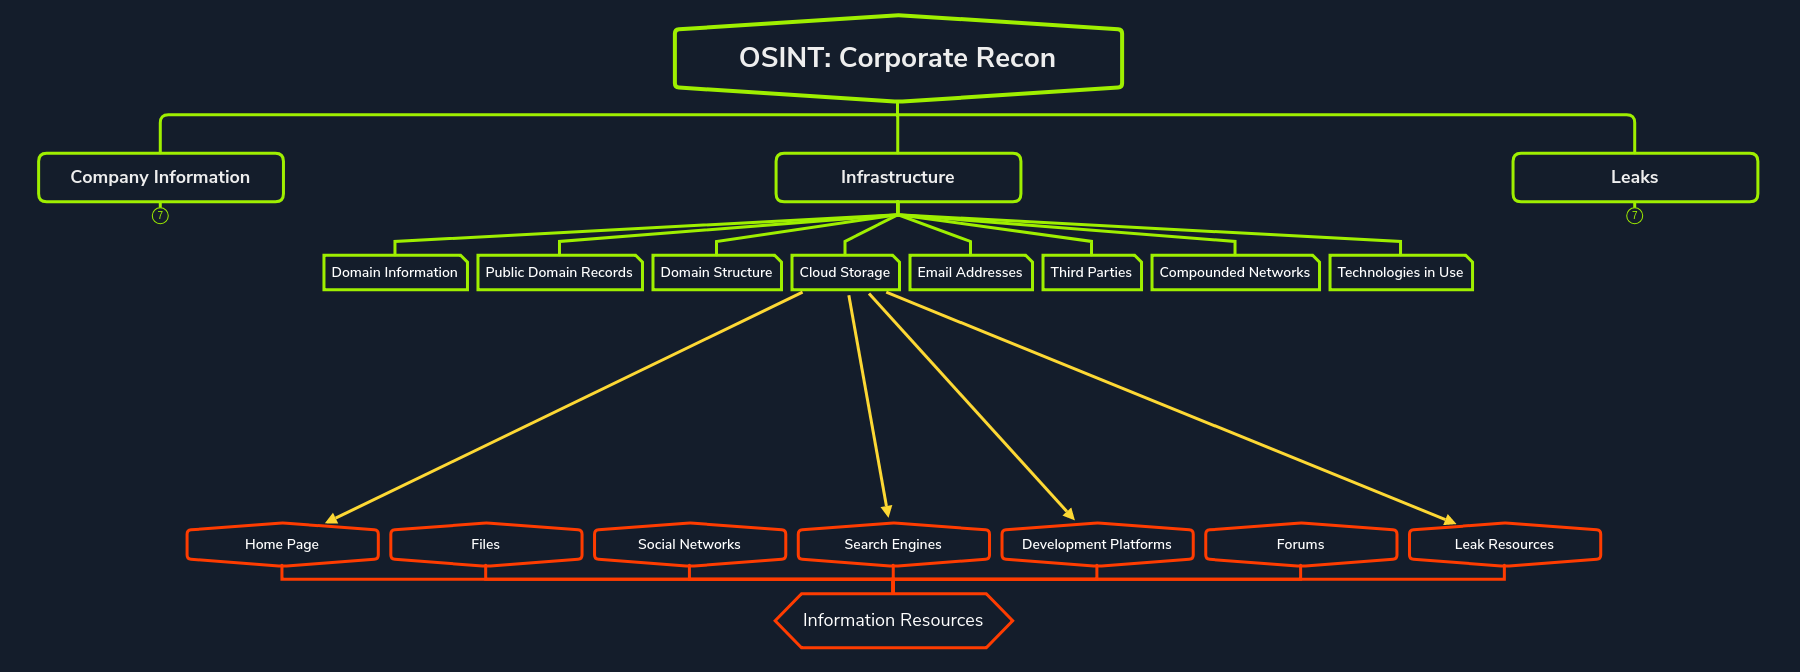
\includegraphics[width=\linewidth]{recon/osint/images/infra-cloud.png}
  \caption{OSINT Infra cloud}
  \label{fig:osint-infra-cloud}
\end{figure}

We can now resolve the domains found into IP addresses and compare them to the
netblocks for these three cloud providers. If we find any IP addresses within
these IP ranges, we can assume that it is a cloud provider. For us, the most
critical component in the corporate use of a cloud provider is open cloud
storage because if they have been misconfigured, they are publicly accessible
and viewable. Some of those cloud providers are, but not limited to:
\begin{verbatim}
 				
Cloud Provider 	    GCP 	                Azure 	    AWS 	    DigitalOcean
Open Cloud Storage 	Google Storage Bucket 	Block Blob 	S3 Buckets 	Spaces
\end{verbatim}

We can also automate this process with the tool
\href{https://github.com/oldrho/ip2provider}{ip2provider.py}. This will
automatically compare the IP addresses with the netblocks and show if they are
successful matches.

\begin{verbatim}
cat Target_Company.IPv4s | ./ip2provider.py
\end{verbatim}

\subsubsection{Home Page}
When searching for cloud buckets, one factor makes it difficult for us to
identify the bucket belonging to the company. This is that everyone can create
their own name for the desired bucket. This means that anyone can create a
bucket with the target company's name without it belonging to the company.

Here we can also find a list of URLs from which we can see which cloud provider
the storage belongs to and where we could find it.

\begin{verbatim}
Cloud Provider 	URL
GCP 	https://www.googleapis.com/storage/v1/b/<bucket-name>/iam

Azure 	https://<bucket-name>.core.windows.net/<container>/
	i   https://<bucket-name>.blob.core.windows.net/<container>/

AWS 	https://<bucket-name>.s3.amazonaws.com
	    https://s3-<region>.amazonaws.com/<company-name>
\end{verbatim}

Almost all (~95\%) vulnerabilities in the cloud happen due to misconfigurations. These misconfigurations include, but are not limited to:
\begin{itemize}
    \item   ACLs
    \item   Bucket Policies
    \item   Service Control Policies
    \item   Public Access Blocks
    \item   IAM Policies
\end{itemize}

Cloud environments extend the penetration testing process enormously. However,
this does not affect the OSINT process since we ultimately use public resources
to not interact with our target company. Further investigation of cloud buckets
will be covered in another Module, as we need to investigate and understand the
setup and the individual configuration options to work with them effectively.
However, we already know enough to find open cloud buckets. Whether they are
open and whether we can see the content on them requires interaction.
Therefore, we will stop after finding them, and in the next stage, we will deal
with them and enumerate them.


The first information resource often used for this purpose is the company's
website. Buckets are often used as a source for the web servers and their
contents are linked accordingly.

We can also use this content and the names of the files or the company's full
domain name (i.e., www-target-company-com) for Searchcode to see if they are
publicly retrievable and if there might even be more information resources for
them. To do this, we take the name of the file and can, for example, look for
other cloud providers to see if they are available there. The more unique the
name of the file is, the more accurate the results will be. These are then
easier to identify and connect to the target company.

\subsubsection{Search Engines}
If files have been tagged or named in conjunction with the company name, we can
use the search engines we know and filter the results based on the cloud
providers. Aside from file names and company names, we may also use employee
names or application names if they appear unique. For this, we can set the
known domains from the cloud providers as the assumed content (with the
\verb+inurl:+ tag) for our results. This will reduce the results only to those
that contain this domain. Finally, we know that the buckets' label will not
necessarily have the name or label we have already seen. For this, search
engines help us to expand our search scope but also to reduce it.

Another information resource that serves very well for finding such buckets is
the \href{https://buckets.grayhatwarfare.com/}{GrayHatWarfare Project}. This
project is an online tool that searches for open cloud buckets and archives
them. This is one of the most widely used tools currently, and it also gives
excellent results since it contains an enormous amount of records.

The GrayHatWarfare Project offers us many different options, such as filtering
by buckets, files, file types, keywords, and even an API interface. We can
search these buckets for files and see which of them might be relevant for us.
The advantage is that we do not have any interaction with buckets owned by the
target company as long as we do not explicitly call the files or list them via
the CLI.

\subsubsection{Development Platforms}

Again, developer platforms are of great use to us, as we can search code to
find out if specific files exist in connection with the cloud buckets. As we
know, {\bf Searchcode} also redirects us to the resource that points to the
corresponding file. Often used strings in these files are {\bf AccountName} and
{\bf AccountKey}, used for authorization (like username and password).

These files usually contain the {\bf IP addresses} or the {\bf bucket names} for the
corresponding cloud storage. We can use these to search again on {\bf
GrayHatWarfare}
and filter out the results. Therefore, if we follow these files and examine
them more closely, we will most likely find a lot more helpful information that
we will need for our documentation and further research. 

\subsubsection{Leak Resources}

Another source that can point us to the buckets and forward them is the
aforementioned \href{https://opendata.rapid7.com/sonar.fdns_v2/}{Rapid7
database}. Since this works with the forward DNS requests and responses and
documents those, it is even very likely that we will find entries that will
show us the corresponding buckets.


\subsection{Email Addresses}

\begin{figure}
  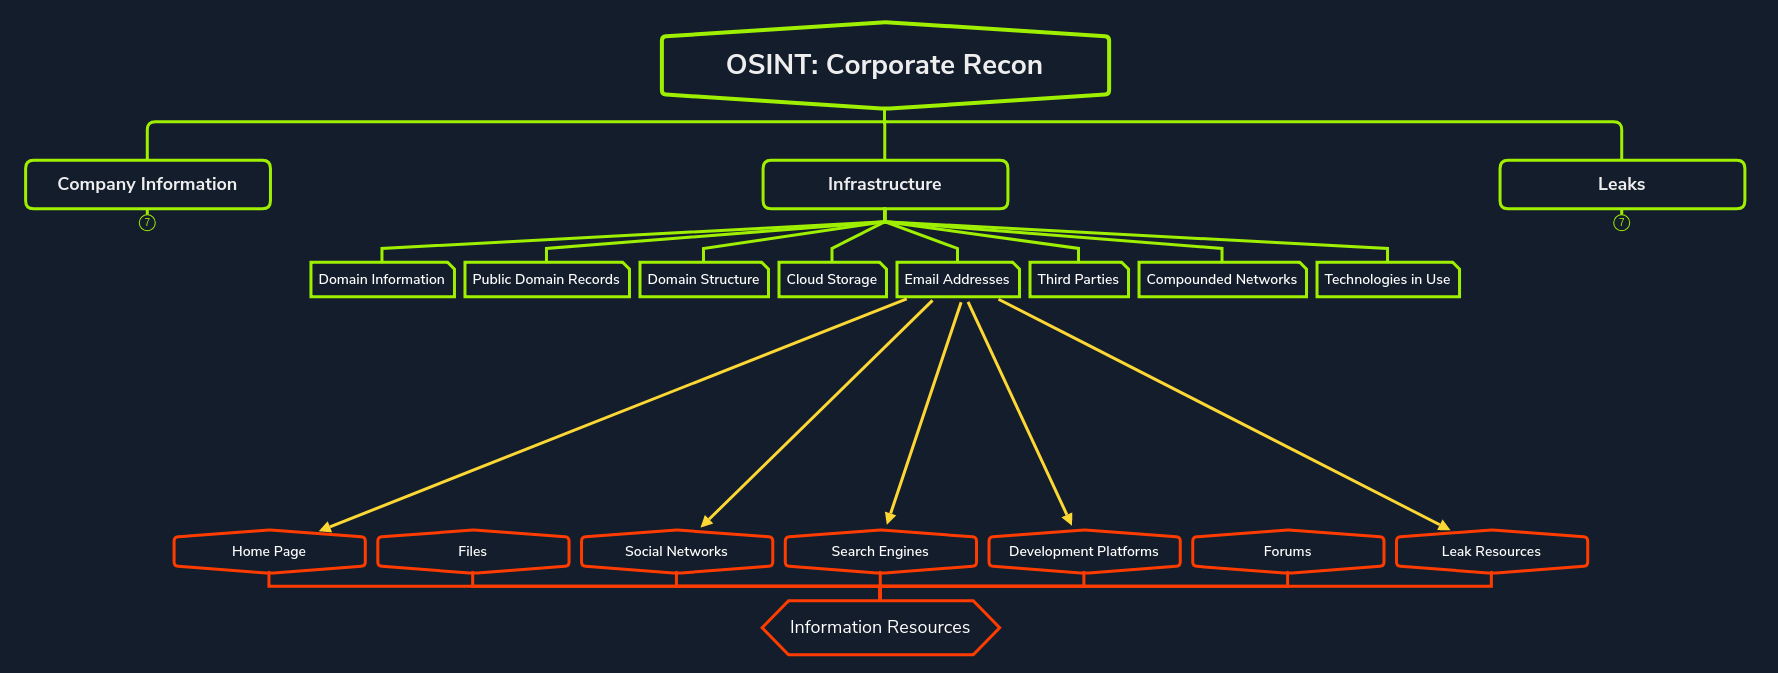
\includegraphics[width=\linewidth]{recon/osint/images/infra-emails.png}
  \caption{OSINT Infra Emails}
  \label{fig:osint-infra-emails}
\end{figure}

